\DiaryEntry{Harmonic Series}{2016-09-12}{Maths}

\subsection{Definition}

The harmonic series is defined as

\[
H_n  = \sum_{k=1}^n \frac{1}{k}
\]

\subsubsection{Divergence}

This series diverges for \(n \rightarrow \infty\) which can be shown as follows: We have

\[
H_\infty = 1 + \frac{1}{2} + \frac{1}{3} + \frac{1}{4} + \frac{1}{5} + \frac{1}{6} + \cdots
\]

which terms we can group according to powers of 2: We put one term into group 1, 2 terms into group 2, 4 terms into group 3 etc.

\[
H_\infty = 1 + \left( \frac{1}{2} + \frac{1}{3} \right) + \left( \frac{1}{4} + \frac{1}{5} + \frac{1}{6} + \frac{1}{7} \right) +  \left( \frac{1}{8} + \frac{1}{9} + \cdots + \frac{1}{15} \right) + \cdots
\]

The two terms in group 2 are between \(1/2\) and \(1/4\), therefore the sum is between \(1/2\) and \(1\). In a similar spirit are the terms of group 3 between \(1/4\) and \(1/8\); therefore the sum is again between \(1/2\) and \(1\). This property holds in general; i.e.~group \(k\) contains the \(2^{k-1}\) elements \(\frac{1}{2^{k-1}}\) and
\(\frac{1}{2^k - 1}\) and the sum of these elements is between \(1/2\) and \(1\).

\subsubsection{Bounds}

From this grouping procedure we obtain two bounds for \(H_n\) (with \(n\) contained in group \(k\)): For an upper bound, we bound the sum of every group by \(1\); then \(H_n \leq k\). For a lower bound, we bound every sum with \(1/2\) and therefore \(H_n > k/2\). Since \(k/2\) diverges for \(k \rightarrow \infty\), also \(H_n \rightarrow \infty\).

By observing that \(k = \lfloor \log_2 n \rfloor + 1\), we can obtain a bound for \(H_n\) in terms of \(n\) as follows

\[
\frac{\lfloor \log_2 n \rfloor + 1}{2} < H_n \leq \lfloor \log_2 n \rfloor + 1
\]

An tighter bound can be obtained by considering the following Figure:

\begin{figure}
\centering
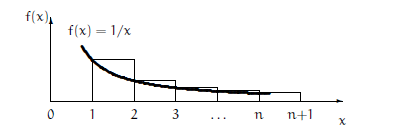
\includegraphics{images/harmonic_series_1.png}
\caption{Page1}
\end{figure}

The are below the curve between \(1\) and \(n\) is \(\int_1^n 1/x dx = \ln n\) is less than the area of the \(n\) rectangles which equals \(\sum_{k=1}^n 1/k = H_n\).

Using slightly different rectangles as shown below

\begin{figure}
\centering
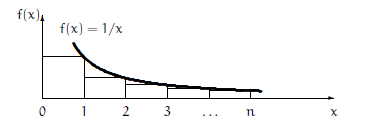
\includegraphics{images/harmonic_series_2.png}
\caption{Page1}
\end{figure}

the rectangle area \(1 + H_n\) is larger than \(\ln n\). Combining, we obtain the following bound

\[
\ln n < H_n < \ln n + 1
\]

\subsubsection{Connection with Euler's Constant}

Riemann's zeta function is defined as

\[
\zeta(r) = H_\infty^{(r)} = \sum_{k=1}^\infty \frac{1}{k^r}
\]

and converges for \(r > 1\) (Note that \(\zeta(1) = H_\infty\)).

Now consider the infinite series

\[
\ln \left( \frac{k}{k-1} \right) = \ln k - \ln(k-1) = \frac{1}{k} + \frac{1}{2k^2} + \frac{1}{3k^3} + \cdots
\]

and sum it from \(k=2...n\). The left side telescopes; i.e.~we have \(\ln 2 - \ln 1 + \ln3 - \ln 2 + \cdots + \ln n - \ln (n-1) = \ln n - \ln 1\). Therefore, we obtain

\[
\ln n - \ln 1 = \sum_{k=2}^n \left( \frac{1}{k} + \frac{1}{2k^2} + \cdots \right) = H_n-1 + \frac{1}{2} (H_n^{(2)}-1) + \frac{1}{3} (H_n^{(3)}-1) + \cdots
\]

We can rearrange this to get the different between \(H_n\) and \(\ln n\) as follows:

\[
H_n - \ln n = 1 - \frac{1}{2} (H_n^{(2)}-1) - \frac{1}{3} (H_n^{(3)}-1) - \cdots
\]

Taking the limit \(n \rightarrow \infty\), the right hand approaches the limiting value

\[
\lim_{n \rightarrow \infty} = 1 - \frac{1}{2} (\zeta(2)-1) - \frac{1}{3} (\zeta(3)-1) - \cdots = \gamma
\]

which is known as Euler's constant, \(\gamma\). Summarizing, we have

\[
\lim_{n \rightarrow \infty} = H_n - \ln n = \gamma
\]

\subsection{$H_n$ is non-integral}

Apart from \(n=1\), \(H_n\) never has an integer value. Even more, any consecutive subseries of \(H_n\), \(Smn = \frac{1}{m} + \cdots \frac{1}{n}\), is never an integer.

However, I do not understand the proof\ldots{}

\subsection{Interesting values}

Just playing around with the numbers:

\[
\begin{array}{cccc}
n & H_n & \ln n & \ln n+1 \\
\hline
1    & 1     & 0     & 1 \\
2    & 1.5   & 0.693 & 1.693 \\
5    & 2.283 & 1.609 & 2.609 \\
10   & 2.929 & 2.303 & 3.303 \\
50   & 4.499 & 3.912 & 4.912 \\
100  & 5.187 & 4.605 & 5.605 \\
1000 & 7.485 & 6.908 & 7.908
\end{array}
\]

Python:

\begin{verbatim}
% n = 1000
sum([1/x for x in range(1,1001)])
\end{verbatim}

\subsection{Application}\label{application}

Overlaying cards, as described in ``Concrete Mathematics'', Section 6.3.
